\documentclass[12pt,a4paper]{article}
\usepackage[utf8]{inputenc}
\usepackage{graphicx}
\usepackage{geometry}
\usepackage{caption}
\usepackage{subcaption}
\usepackage{hyperref}
\usepackage{booktabs}

\geometry{
  top=1in,
  bottom=1in,
  left=1in,
  right=1in
}

\title{Contextual Bandit Routing in LLM Applications}
\author{ParetoBandit Blog}
\date{\today}

\begin{document}

\maketitle

\begin{abstract}
As the complexity of applications powered by Large Language Models (LLMs) increases, managing the trade-off between cost, quality, and processing time becomes paramount. This document illustrates a complete framework for integrating a Contextual Bandit Router: session-level routing for direct user interactions (such as a career coach application), sub-task routing within autonomous agentic systems, expert selection in multi-agent architectures, hierarchical routing (Orchestrator $\rightarrow$ Agent $\rightarrow$ Bandit $\rightarrow$ LLM), latency-aware routing, mitigating router overhead, a complexity comparison between Macro and Micro routing strategies, and finally, the profound business case for dense programmatic rewards. By dynamically selecting the optimal model based on context and historical rewards, these routers approach frontier-level helpfulness at significantly reduced average costs and latencies, empowering specialized agents to run cost-effective internal pipelines.
\end{abstract}

\section{Introduction: Why Agents Make Many LLM Calls}

A common misconception is that an AI ``agent'' is simply a wrapper around a single LLM call. In reality, every major agent framework---LangChain, LlamaIndex, CrewAI, AutoGen, and the OpenAI Assistants API---implements a \textbf{loop}, not a single call. The standard pattern, known as ReAct (Reason-Act-Observe), works as follows:

\begin{enumerate}
    \item \textbf{Think:} The agent calls an LLM to reason about what to do next.
    \item \textbf{Act:} The agent executes a tool (e.g., search the web, query a database, parse a PDF).
    \item \textbf{Observe:} The agent receives the tool's output.
    \item \textbf{Think again:} The agent calls an LLM \textit{again} to interpret the tool output and decide the next step.
    \item Repeat until the task is complete.
\end{enumerate}

A single ``atomic'' agent answering one user question might make 3--10 LLM calls just to complete one task. A complex research agent might make 20--50 calls in a single session. Crucially, \textbf{not all of these calls require the same level of reasoning power}. A planning step (``I need to extract text from this PDF'') is a trivial thought that any small model can handle. A deep analysis step (``Compare these resume keywords against the job description and identify gaps'') genuinely requires a powerful reasoning model.

Without a Contextual Bandit, every framework defaults to calling the \textit{same model} for all of these steps. The engineer picks one model in a configuration file, and that model handles everything---planning, tool interpretation, reasoning, and generation alike. This creates a forced choice between a cheap-but-unreliable agent and an expensive-but-slow agent.

A Contextual Bandit Router, placed \textit{inside} the agent, breaks this assumption. It learns which internal steps can use the fast, cheap model and which ones truly need the expensive reasoning model---automatically, from programmatic success/failure signals, without any human labeling. This document explores the full spectrum of where and how to deploy such routers, from simple session-level routing to deep intra-agent optimization.

\section{Session-Level Routing: The Career Coach}

In a direct user-facing application, such as a career coaching app, users bring diverse intents. A user might ask for a simple task, like ``Practice salary negotiation,'' or a complex one, like ``Plan a career change.'' A Contextual Bandit Router evaluates the context of each incoming session and dynamically assigns it to the most appropriate LLM.

Figure \ref{fig:bandit_router} illustrates this architecture. The router learns from historical user feedback (e.g., 5-star ratings) to map specific session types to either a small (low-cost), medium, or large (high-cost) model. Over time, the router builds a Pareto-optimal frontier, ensuring that simple queries are handled cheaply without sacrificing quality, while complex queries receive the necessary reasoning power.

\begin{figure}[h]
    \centering
    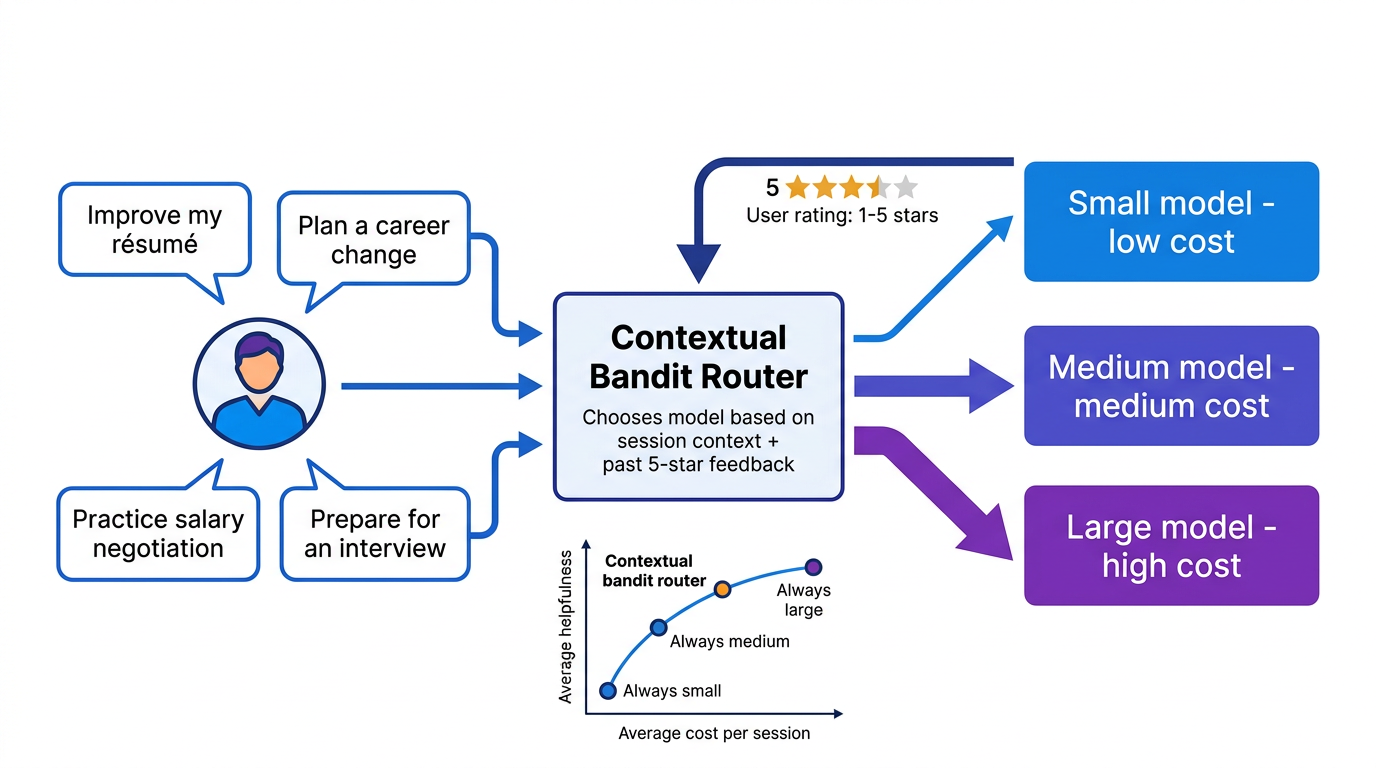
\includegraphics[width=\textwidth]{bandit_router_infographic.png}
    \caption{A contextual bandit router learns from 5-star user feedback which LLM (small, medium, or large) to use for each career-coaching session type, approaching frontier-level helpfulness at a much lower average cost.}
    \label{fig:bandit_router}
\end{figure}

\section{Sub-Task Routing: Agentic Systems}

When deployed within an autonomous agentic system, the Contextual Bandit Router becomes a dynamic sub-task optimizer. Agents break complex goals down into numerous internal steps: planning, tool use (e.g., web search), data extraction, and synthesis. 

As shown in Figure \ref{fig:agentic_router}, rather than routing a monolithic prompt, the orchestrator routes these internal thought processes. For instance, complex planning might require a Large Model, while simple data extraction or formatting can be reliably performed by a Small Model. The reward signal here shifts from human ratings to programmatic environmental feedback—such as whether a tool call executed without syntax errors or if the output was valid JSON. This fine-grained optimization drastically reduces the cost of running thousands of agent iterations.

\begin{figure}[h]
    \centering
    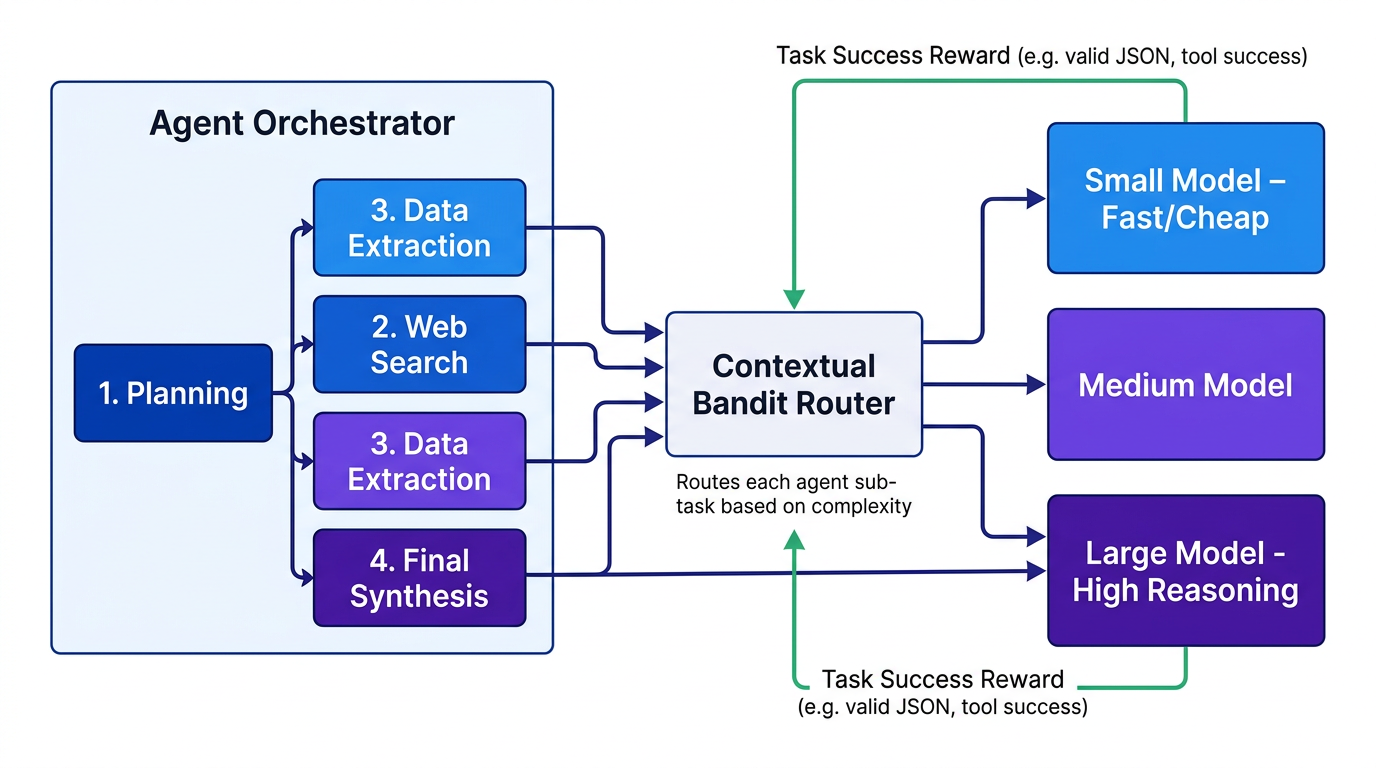
\includegraphics[width=\textwidth]{agentic_bandit_router.png}
    \caption{In an agentic workflow, a contextual bandit router dynamically assigns sub-tasks (Planning, Web Search, Data Extraction) to the most cost-effective model, learning from programmatic success metrics rather than direct human feedback.}
    \label{fig:agentic_router}
\end{figure}

\section{Agent Routing: The Multi-Agent Orchestrator}

In a multi-agent system where different LLMs or specialized prompt pipelines are designated as experts (e.g., General FAQ, Communication Coach, Resume Writer, Salary Negotiator), the Contextual Bandit Router acts as a central triage system called the ``Head Coach.''

Crucially, different expert agents incur vastly different operational costs. A General FAQ Agent might require a single prompt to a fast, cheap model, whereas a Salary Negotiator Agent might execute a complex loop involving deep web searches, data parsing, and a massive reasoning model. Even worse, if an agent completely fails, the system might have to escalate the session to an expensive human coach. 

When a user presents an ambiguous query—such as ``I keep freezing up when they ask about my past projects''—the router must determine which specialized expert agent is best equipped to handle the session without overspending. 

As illustrated in Figure \ref{fig:multi_agent}, the router evaluates the session context (e.g., the user is in the ``Final Round'' and their tone is ``Anxious'') and dispatches the query to the Communication Coach Agent. The reward signal here is a composite of ``Resolution Success'' and ``Compute Cost.'' Did the selected expert help the user achieve their goal, and did it do so efficiently? Over time, the Contextual Bandit learns the nuanced mapping between ambiguous user intents and the most cost-effective specialized agent.

\begin{figure}[h]
    \centering
    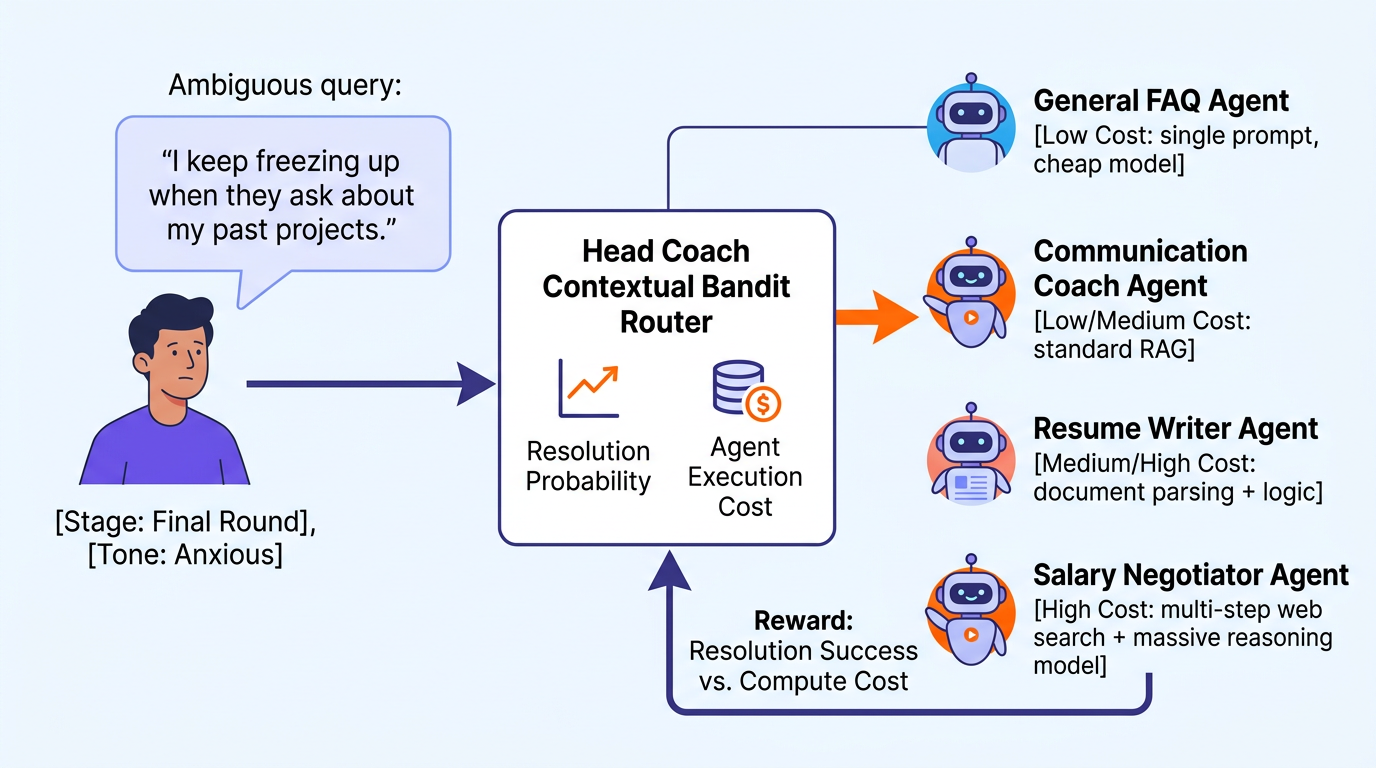
\includegraphics[width=\textwidth]{multi_agent_bandit.png}
    \caption{In a multi-agent architecture, a Contextual Bandit ``Head Coach'' acts as an intelligent triage system, directing ambiguous user queries to the expert agent that maximizes resolution probability while minimizing execution costs.}
    \label{fig:multi_agent}
\end{figure}

\section{Hierarchical Routing: Orchestrator vs. Contextual Bandit}

A common misconception is treating the Orchestrator and the Contextual Bandit Router as the same entity. In an optimal multi-agent architecture, they operate at two distinct levels of abstraction, creating a powerful hierarchical routing system.

At the macro-level, the \textbf{Orchestrator} handles \textit{functional routing}. Its goal is intent classification: recognizing that ``I need help with my resume'' belongs to the Resume Agent, while ``Let's do a mock interview'' belongs to the Interview Agent. It ensures the query is handed to the agent equipped with the correct tools.

At the micro-level, the \textbf{Contextual Bandit} handles \textit{compute routing}. Once the Resume Agent takes over, it executes a workflow of atomic steps (e.g., Extract Text, Analyze Keywords, Fix Grammar). For every single one of these atomic steps, an internal Contextual Bandit decides which LLM API to call. It might route ``Extract Text'' to a fast, cheap model, but route ``Analyze Keywords'' to a massive, expensive reasoning model.

As shown in Figure \ref{fig:hierarchical}, this hierarchical design is critical because the agents themselves are black boxes to the orchestrator. By placing the Contextual Bandit \textit{inside} the atomic agents, the system optimizes at the exact point where compute is spent, drastically lowering the total operational cost of the agent while maintaining high quality.

\begin{figure}[h]
    \centering
    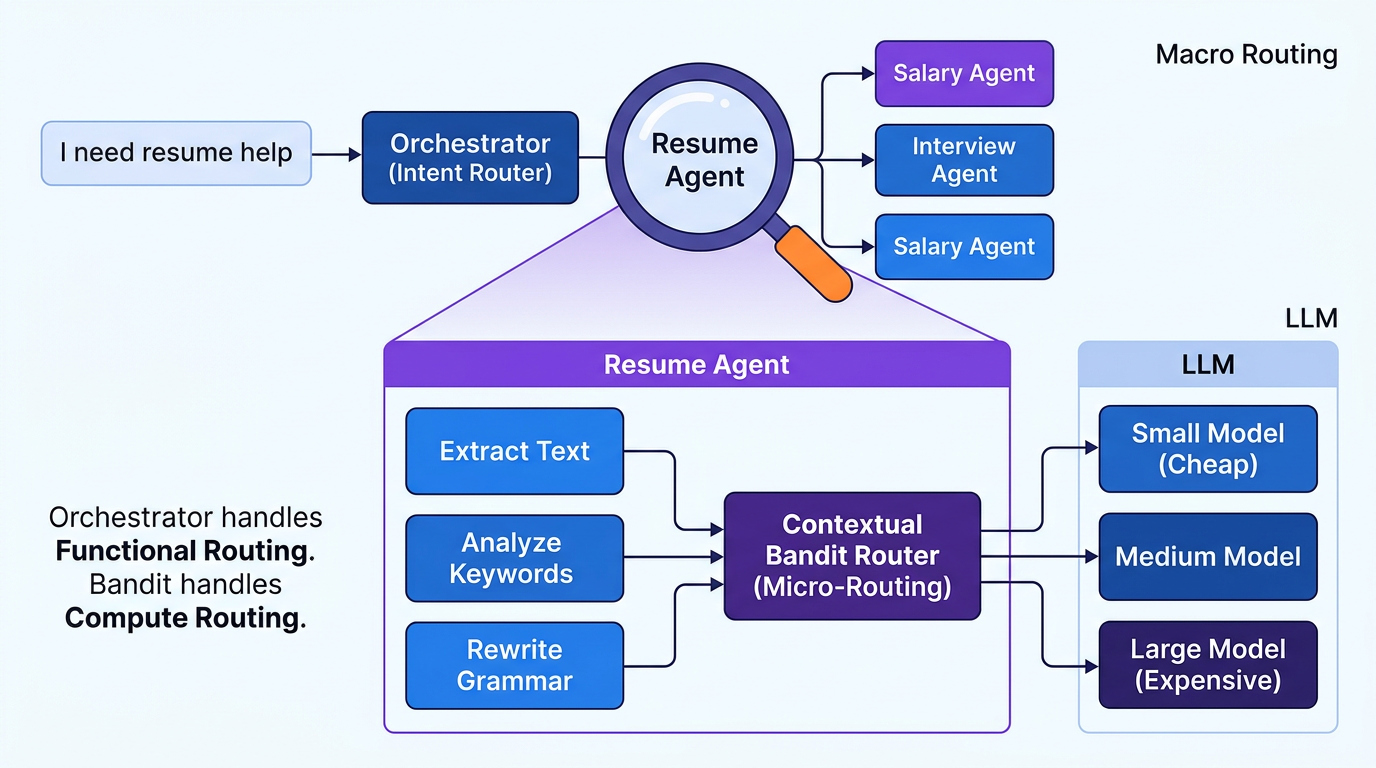
\includegraphics[width=\textwidth]{hierarchical_bandit_router.png}
    \caption{Hierarchical Routing Architecture: The Orchestrator handles macro-level functional routing to specialized agents, while the Contextual Bandit resides inside the agents to handle micro-level compute routing across different LLMs for atomic tasks.}
    \label{fig:hierarchical}
\end{figure}

\section{Latency-Aware Routing: The Processing Time Dimension}

In real-world applications, cost and quality are not the only determining factors of success; \textbf{processing time} (latency) is often the hard constraint that defines user experience. A Contextual Bandit is perfectly suited to handle this by treating latency as an explicit, dynamic penalty in its reward function.

Instead of a simple trade-off, the bandit solves a multi-objective optimization problem, typically structured as:
$$ Reward = Quality - (\alpha \times Cost) - (\beta \times Latency) $$

Crucially, the latency penalty weight ($\beta$) is not static—it is determined by the session context. As illustrated in Figure \ref{fig:latency}, consider two different user interactions within the career coach app:

\begin{enumerate}
    \item \textbf{Synchronous / Real-Time Context:} A user is doing a live Voice Mock Interview. The context demands a Time-To-First-Token (TTFT) of under 500ms to feel natural. The bandit identifies this real-time context and assigns a massive penalty to latency (a high $\beta$). It routes the audio-transcription and response-generation to a blazing-fast, smaller model. It learns that sacrificing a tiny fraction of reasoning quality is mathematically required to maximize the user's reward.
    \item \textbf{Asynchronous / Offline Context:} A user uploads their 5-page resume and requests a comprehensive ``Career Strategy Report,'' which will be emailed to them later. The latency penalty ($\beta$) drops to near-zero. The bandit realizes it has a massive time budget and routes the task to a slow, heavy-reasoning model that might take 45 seconds to process, ensuring the highest possible quality.
\end{enumerate}

By feeding the system's time constraints into the state vector, the Contextual Bandit seamlessly toggles between optimizing for speed and optimizing for depth.

\begin{figure}[h]
    \centering
    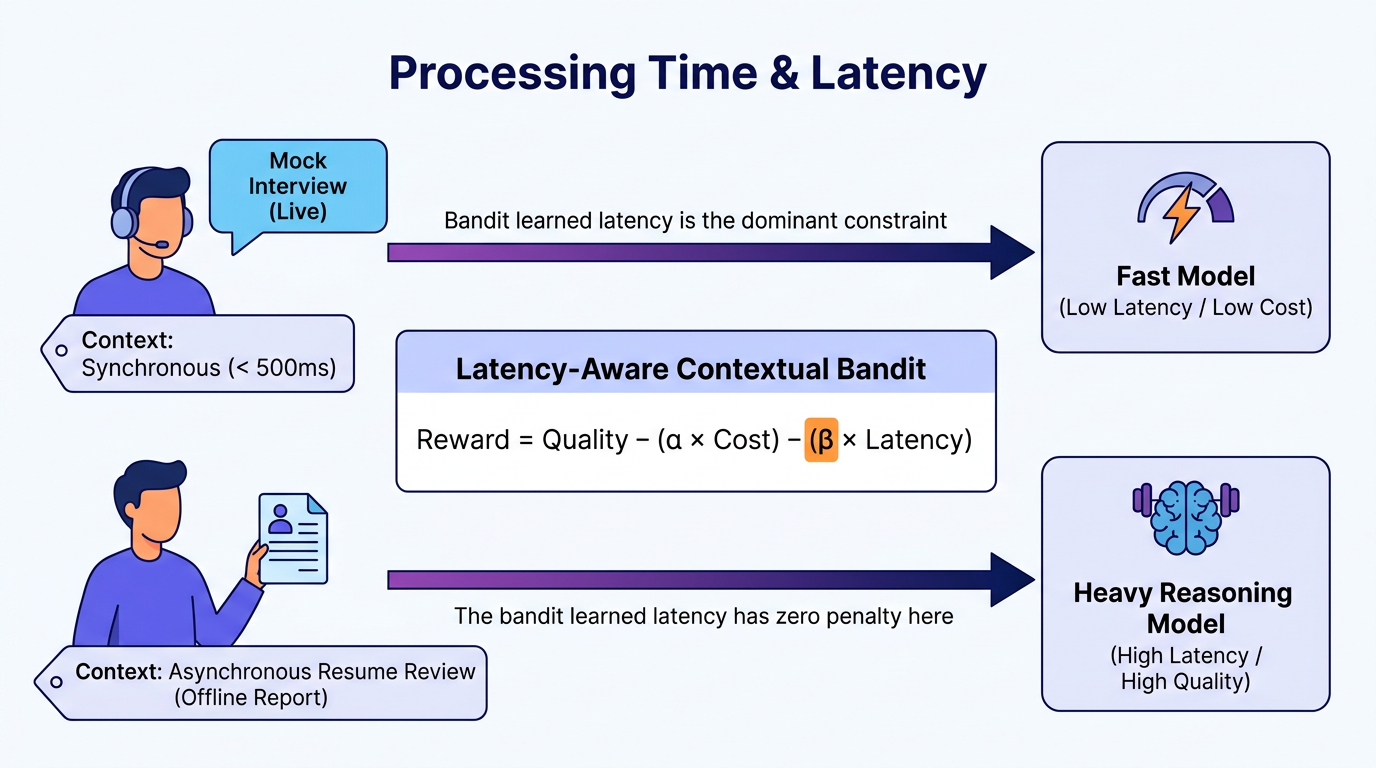
\includegraphics[width=\textwidth]{latency_bandit_router.png}
    \caption{Latency-Aware Routing: The Contextual Bandit dynamically adjusts the penalty for processing time based on whether the user's interaction is synchronous (e.g., live voice chat) or asynchronous (e.g., an offline report generation), directing queries to fast models or heavy reasoning models accordingly.}
    \label{fig:latency}
\end{figure}

\section{Mitigating Router Overhead: Strategic vs. Atomic Routing}

A critical engineering reality when implementing Contextual Bandits—especially at the micro-routing level inside agents—is \textbf{Router Overhead}. If the bandit evaluates context by making an LLM call itself, or if the bandit is a remote microservice, every single routing decision adds network latency.

Consider a common agentic pattern: ``Chunking and Looping.'' When a Resume Agent receives a 5-page document, it cannot process the entire text at once without risking hallucinations or lost details. Instead, the agent breaks the resume down into 50 individual bullet points and uses a \texttt{for-loop} to check the grammar of each one. 

If you place a Contextual Bandit directly inside that loop, the agent will make 50 separate network calls to the Bandit API just to ask, ``Which LLM should I use for \textit{this specific sentence}?'' If the Bandit API adds 50ms of overhead per call, this naive \textbf{Atomic Routing} approach injects 2.5 seconds of pure ``routing latency'' into the user's wait time—completely defeating the point of optimizing for speed!

To solve this, system designers must implement \textbf{Workflow-Level Policy Routing}. 

As illustrated in Figure \ref{fig:overhead}, instead of asking the bandit for routing instructions 50 times during the loop, the agent evaluates the entire document \textit{once} at the start of the session: ``I just received a 5-page resume with high complexity. What is my routing policy?'' 

The bandit returns a comprehensive \textbf{Workflow Blueprint}:
\begin{itemize}
    \item \textit{Task A (Format Extraction)} $\rightarrow$ Small Model
    \item \textit{Task B (Deep Keyword Analysis)} $\rightarrow$ Large Model
    \item \textit{Task C (Grammar Loop)} $\rightarrow$ Small Model
\end{itemize}

The agent then executes the 50-step loop locally using the prescribed Small Model, incurring \textbf{zero} extra routing latency. Additional strategies include embedding the bandit's inference directly into the agent's memory space (e.g., as a lightweight ONNX model executing in $<1$ ms) and only utilizing the bandit for the most computationally expensive bottlenecks in the pipeline.

\begin{figure}[h]
    \centering
    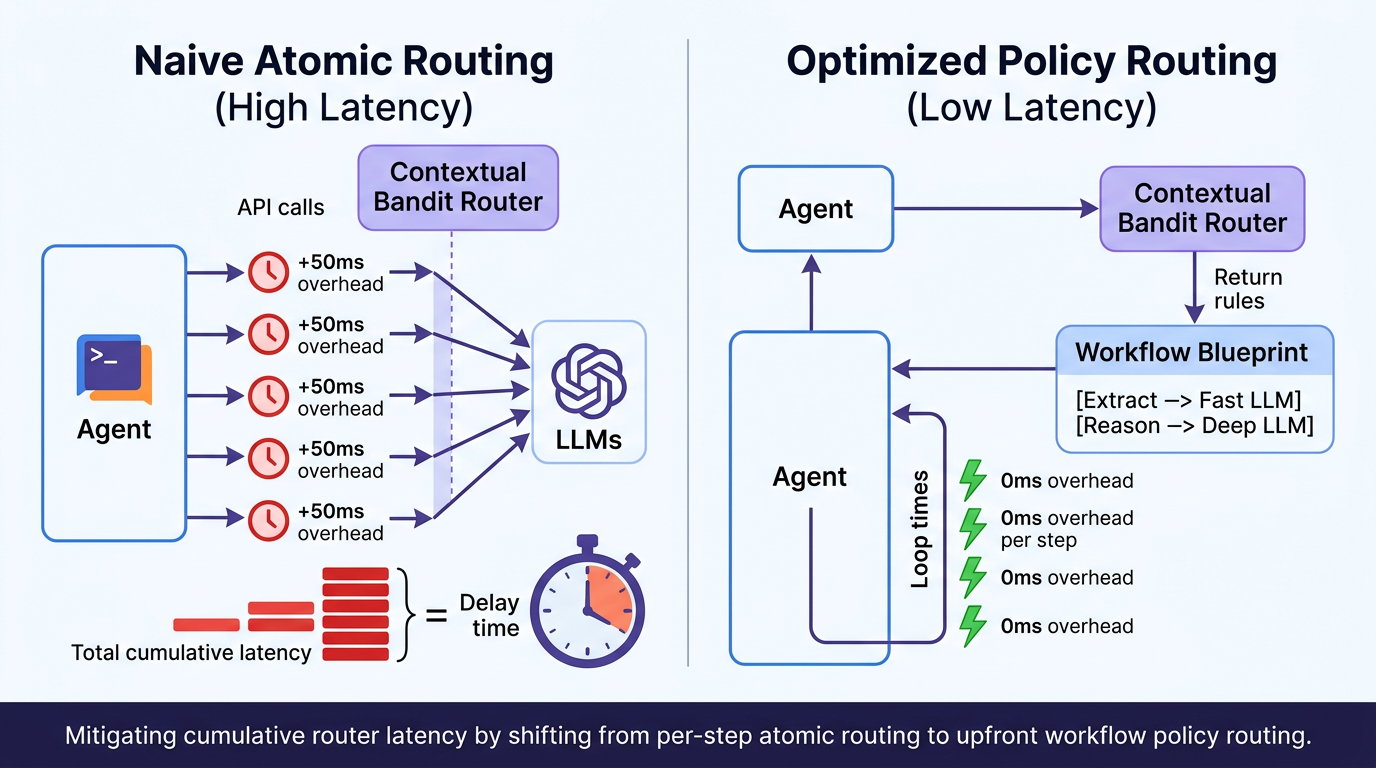
\includegraphics[width=\textwidth]{latency_overhead_mitigation.png}
    \caption{Router Overhead Mitigation: By shifting from per-step naive atomic routing (which suffers from cumulative network latency) to upfront workflow policy routing, the agent eliminates routing overhead during repetitive internal loops.}
    \label{fig:overhead}
\end{figure}

\section{Architectural Complexity: Macro vs. Micro Routing}

A critical architectural decision when designing these systems is determining exactly \textit{where} the Contextual Bandit should sit in your stack. Should it act as the Macro-Orchestrator routing to agents, or as the Micro-Router inside the agents? As illustrated in Figure \ref{fig:comparison}, these two approaches have inverted complexity profiles, specifically regarding the \textbf{Credit Assignment Problem}.

\subsection{Macro-Routing: The Bandit as Orchestrator}
In this approach, the user submits a prompt, and the Bandit sits at the very front of the application, acting as the gateway that selects the expert agent (e.g., Resume Agent vs. Interview Agent).
\begin{itemize}
    \item \textbf{System Complexity (Low):} It is architecturally simple—just an API gateway sitting in front of your tools.
    \item \textbf{Learning Complexity (High):} This approach suffers from massive \textit{reward sparsity}. If the chosen agent takes 20 steps to finish a task and the user gives the final result a 1-star review, the Bandit has no idea \textit{why}. Was it routed to the wrong agent? Did step 14 inside the agent fail? The feedback loop is muddy.
    \item \textbf{When to Use:} Best for simple systems, single-step chat interactions (like LMSYS Chatbot Arena), or environments where agents are closed-source black boxes and subjective user feedback is your only signal.
\end{itemize}

\subsection{Micro-Routing: The Bandit Inside the Agent}
In this approach, a deterministic router (like LangChain or a semantic classifier) acts as the Orchestrator, passing the intent to the Resume Agent. The Resume Agent then uses a Contextual Bandit internally to pick which LLM processes each of its atomic sub-tasks.
\begin{itemize}
    \item \textbf{System Complexity (High):} You must deeply instrument your agent's internal loops, manage workflow blueprints, and handle local inference to avoid router overhead. You are effectively building a custom OS scheduler for AI.
    \item \textbf{Learning Complexity (Low):} The Bandit learns incredibly fast because it gets \textit{programmatic, dense rewards}. When it routes a ``data extraction'' task to a small model, the agent can immediately check: Did the output parse as valid JSON? If yes, Reward = +1. The Bandit learns instantly without waiting for human feedback.
    \item \textbf{When to Use:} Best for complex, multi-step agentic workflows where compute costs are spiraling out of control because agents are naively calling heavy reasoning models for trivial data-munging steps. This is strictly for high-volume, mature production systems.
\end{itemize}

\begin{figure}[h]
    \centering
    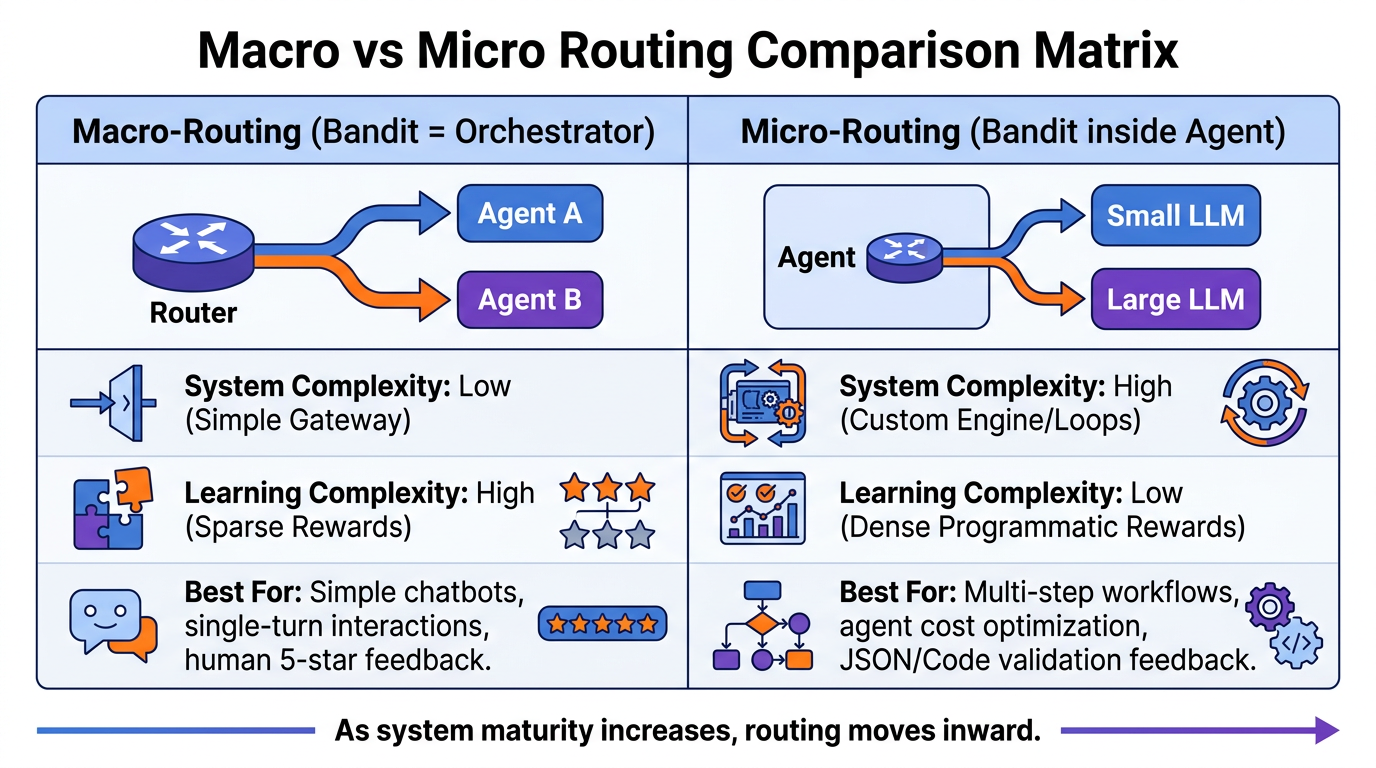
\includegraphics[width=\textwidth]{routing_comparison_matrix.png}
    \caption{Macro vs. Micro Routing: As an AI system matures from simple chatbots to complex multi-step agents, the Contextual Bandit is often pushed further down the stack—trading higher system engineering complexity for incredibly dense, programmatic learning signals.}
    \label{fig:comparison}
\end{figure}

\section{The Business Case for Micro-Routing: Dense Rewards and Margins}

Given the immense engineering complexity of instrumenting internal loops, managing workflow blueprints, and eliminating router overhead, why do companies spend months building Micro-Routing? The justification comes down to two things: \textbf{The Math of Learning} and \textbf{The Math of Business}.

\subsection{The Math of Learning: Sparse vs. Dense Rewards}
Consider an agent that performs 20 atomic steps to draft a complex cover letter. 
\begin{itemize}
    \item \textbf{Macro-Routing (Sparse Rewards):} The user receives the final cover letter and rates it 2 stars. The Bandit receives a $-1$ penalty. But \textit{why}? Did the PDF extractor fail? Was the tone off? Did the JSON formatting break? The Bandit doesn't know. It might take 10,000 interactions to statistically guess the failure point. This is sparse, noisy feedback.
    \item \textbf{Micro-Routing (Dense Rewards):} The Bandit is inside the agent picking models step-by-step. In Step 1 (Extract), it picks a cheap model, the code verifies text was returned, and the Bandit instantly gets a $+1$. In Step 5 (Format JSON), it picks a cheap model, the Python script gets a \texttt{SyntaxError}, and the Bandit instantly gets a $-1$. In a single session, without waiting for the human to do anything, the micro-bandit gathers 20 objective, programmatic data points.
\end{itemize}

As shown in Figure \ref{fig:rewards}, dense rewards allow the system to learn the exact boundaries of what small models can and cannot do in minutes rather than months.

\begin{figure}[h]
    \centering
    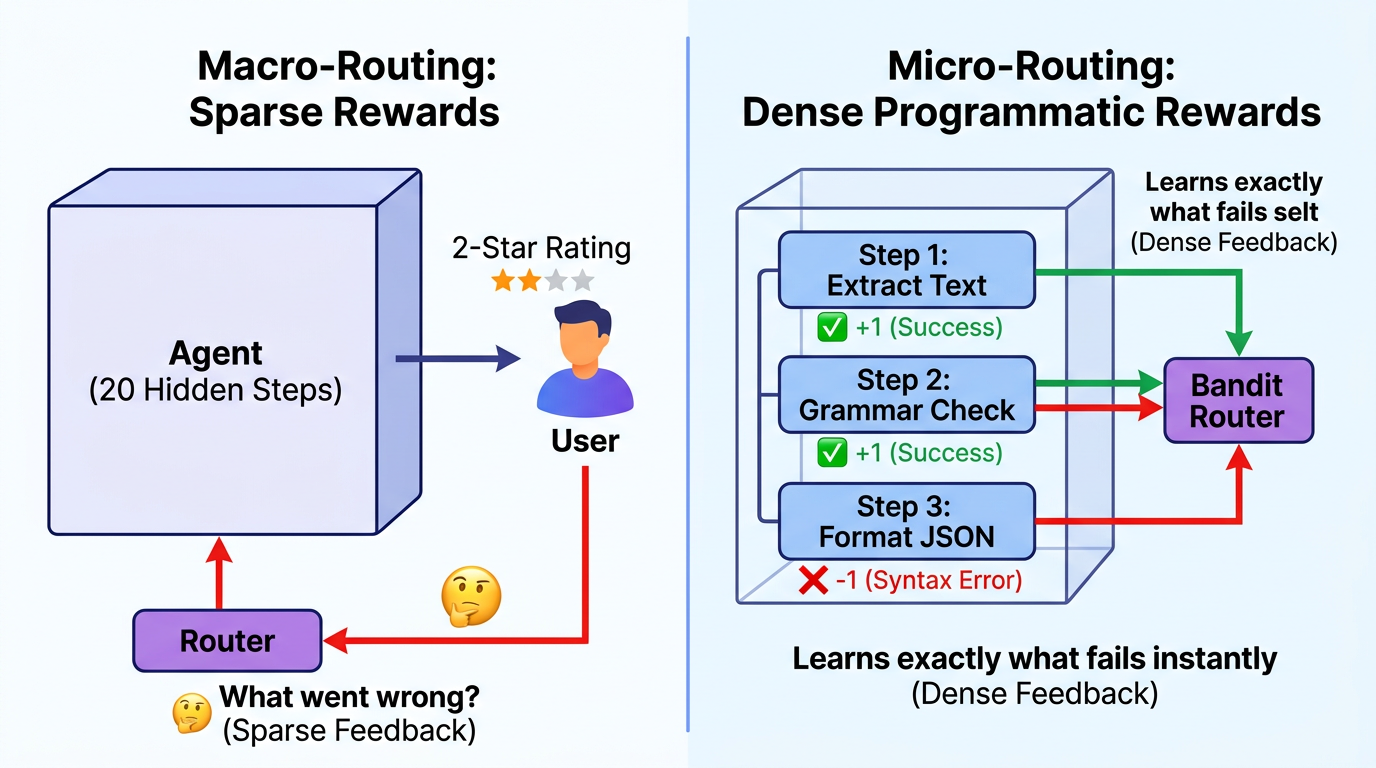
\includegraphics[width=\textwidth]{sparse_vs_dense_rewards.png}
    \caption{Sparse vs. Dense Rewards: Macro-routing relies on single, delayed human feedback signals (sparse), while Micro-routing generates instant, programmatic success/failure signals for every internal step (dense).}
    \label{fig:rewards}
\end{figure}

\subsection{The Math of Business: Gross Margins}
If you build an agent without micro-routing, you face a brutal dilemma:
\begin{itemize}
    \item \textbf{The ``Cheap'' Agent:} You hardcode the agent to use a $0.05$ model for all 20 steps. It fails at complex reasoning 30\% of the time. Customers churn.
    \item \textbf{The ``Premium'' Agent:} You hardcode the agent to use a massive $2.00$ reasoning model for all 20 steps to ensure success. The app is slow, API costs destroy your gross margins, and you cannot scale profitably.
\end{itemize}

The Micro-Routing Contextual Bandit solves this. It learns to use the $0.05$ model for the 18 easy steps (extraction, formatting) and the $2.00$ model \textit{only} for the 2 steps that require genius-level reasoning. 

From the company's view, the blended API cost drops to $0.25$ per session, improving gross margins by 8x. From the customer's view, the app is incredibly fast (due to the 18 fast models), highly reliable, and far more affordable. This is why Micro-Routing is the architectural end-state for mature AI products.

\section{Conclusion}

Whether operating at the session level for direct user queries, at the sub-task level within agent orchestrations, acting as the central dispatcher in a multi-agent expert system, or functioning hierarchically as the internal compute-router for specialized agents, Contextual Bandit Routers offer a robust framework. By continuously learning from explicit or implicit reward signals, they ensure that expensive reasoning capabilities are deployed efficiently, lowering the operational floor while raising the quality ceiling of modern AI architectures.

\appendix
\section{Worked Example: LLM Calls Inside a Resume Agent}
\label{app:resume_walkthrough}

To make the case for intra-agent bandit routing concrete, Table \ref{tab:resume_agent} traces every LLM call that a Resume Agent makes when a user submits ``Review my resume against this job posting.'' Without a Contextual Bandit, every step uses the same model. With a bandit, each step is routed to the most cost-effective model that can reliably complete it.

\begin{table}[h]
\centering
\small
\begin{tabular}{@{}clccc@{}}
\toprule
\textbf{Step} & \textbf{Agent Action} & \textbf{LLM Call?} & \textbf{Difficulty} & \textbf{Bandit Routes To} \\
\midrule
1 & Plan: ``I need to extract text'' & Yes & Trivial & Small Model \\
2 & Execute: Call PDF extraction tool & No & --- & --- \\
3 & Plan: ``Now compare keywords'' & Yes & Trivial & Small Model \\
4 & Execute: Call web search for job post & No & --- & --- \\
5 & Reason: Compare resume vs. job keywords & Yes & Hard & Large Model \\
6 & Plan: ``Fix grammar in 30 bullets'' & Yes & Trivial & Small Model \\
7--36 & Execute: Fix grammar (30$\times$ loop) & Yes (30$\times$) & Trivial & Small Model \\
37 & Synthesize: Write personalized summary & Yes & Hard & Large Model \\
38 & Format: Output final JSON & Yes & Trivial & Small Model \\
\bottomrule
\end{tabular}
\caption{Anatomy of a single Resume Agent session. Out of 36 total LLM calls, only 2 require the expensive reasoning model. A Contextual Bandit learns this distribution automatically from step-level programmatic feedback (e.g., did the JSON parse? did the keyword comparison pass a coverage threshold?), without any human labeling.}
\label{tab:resume_agent}
\end{table}

\noindent \textbf{Cost comparison for this single session:}
\begin{itemize}
    \item \textbf{Without bandit (all Large Model):} 36 calls $\times$ \$0.06/call = \textbf{\$2.16}
    \item \textbf{Without bandit (all Small Model):} 36 calls $\times$ \$0.001/call = \textbf{\$0.04}, but Steps 5 and 37 fail 30\% of the time
    \item \textbf{With bandit (mixed routing):} 34 calls $\times$ \$0.001 + 2 calls $\times$ \$0.06 = \textbf{\$0.15}, with near-zero failure rate
\end{itemize}

This pattern generalizes across every agent in a multi-agent system. Each specialized agent (Interview Prep, Communication Coach, Salary Negotiator) has its own internal loop of LLM calls, and each benefits from a Contextual Bandit that learns the difficulty profile of its specific workflow. The compounding savings across all agents and all users is what transforms Micro-Routing from an engineering curiosity into a business-critical capability.

\end{document}
